\documentclass{book}
\usepackage{blindtext}
\usepackage[T1]{fontenc}
\usepackage[polish]{babel}
\usepackage[utf8]{inputenc}
\usepackage{listings}
\usepackage{graphicx}
\usepackage{float}
\usepackage{multirow}
\usepackage{hyperref}
\graphicspath{ {./Wykresy/} }


\title{Analiza wpływu zastosowania wybranych technik przygotowania danych do analizy, na jakość analizy danych}
\author{Dariusz Litwiński}
\date{\today}

\renewcommand\lstlistingname{Przykład}

\begin{document}
\maketitle
\chapter{Problem Analizy Danych}

\section{Analiza Danych}
Analiza danych to proces, 
w którym przekształcamy surowe dane w wiedzę i 
wnioski, dzięki którym jesteśmy w stanie podejmować lepsze decyzje \cite{data_analysis}. 
Wewnątrz tego procesu można wyróżnić następujące fazy:

\subsection{Pozyskiwanie: gromadzenie danych}
Zanim analiza danych będzie możliwa należy pozyskać dane, 
jest to istotna cześć procesu, ponieważ to od niej zależy to, 
jak trafne wnioski będziemy mogli wysnuć na późniejszych etapach.
Bardzo ważne jest to, jak dużą ilość danych uda nam się zebrać, a także jak dokładne one będą.
Możemy pozyskiwać dane z różnorakich źródeł, na przykład: 
\begin{itemize}
    \item Zapisywać wartości zbierane przez czujniki 
    \item Korzystać z ankiet wśród danej populacji
    \item Zbierać dane o zachowaniach użytkowników w trakcie korzystania ze strony internetowej
  \end{itemize}
Jesteśmy w tej kwestii ograniczeni jedynie przez dziedzinę, w jakiej przeprowadzamy analizę danych
Istotną kwestią jest również to, w jakim formacie są 
przechowywane dane. Może okazać się, że pierwszym etapem przetwarzania danych 
będzie odpowiednie ich sformatowanie, bądź nawet ich cyfryzacja, jeśli były 
by przechowywane w formie fizycznej, na przykład jako papierowe archiwa


\subsection{Przygotowanie: przetwarzanie danych}
Aby móc w pełni korzystać ze zgromadzonych danych, 
należy je przygotować, odpowiednio sformatować. 
Poza przygotowaniem odpowiedniego formatu danych, 
możemy wyróżnić następujące sposoby na przygotowanie danych do analizy:
\begin{itemize}
    \item Wypełnienie brakujących wartości 
    \item Standaryzacja danych liczbowych
    \item Kodowanie wartości kategorycznych jako liczbowe
  \end{itemize}
Dzięki wykorzystaniu powyższych sposobów możemy znacznie zwiększyć jakość analizy danych, 
a co za tym idzie wnioski do których dojdziemy w trakcie procesu będą 
trafniejsze i przyniosą lepsze rezultaty


\subsection{Analiza: modelowanie danych}
Mając do dyspozycji przygotowane dane możemy przejść do ich właściwej analizy, 
na podstawie której tworzymy modele, klasyfikatory, systemy rekomendacji, dokonujemy klasteryzacji. 
Najczęsciej nie tworzymy ich od zera, a wspomagamy się dostępnymi bibliotekami, które zawierają 
najpopularniejsze algorytmy. Zdarza się, że nie jesteśmy zadowoleni z wyników, jakie przynosi 
wykorzystanie stworzonych modeli, bądź chcielibyśmy dokonać dalszej optymalizacji czasowej, 
w takim przypadku możemy rozważyć dodatkowe przygotowanie danych, aby uzyskać pożądany efekt.
Po dobrze przeprowadzonej analizie, jesteśmy w stanie 
wykorzystać stworzone na tym etapie narzędzia do rozwiązywania rzeczywistych problemów.

\subsection{Działanie: podejmowanie decyzji}
Mając gotowe narzędzia będące wynikiem modelowania danych, możemy je wykorzystać aby podjąć 
konkretne decyzje w prawdziwym świecie: Wykorzystać stworzony 
klasyfikator w diagnostyce chorób, wdrożyć system rekomendacji 
na naszej stronie internetowej, wykorzystać stworzone klastry danych do kategoryzacji klientów. 
Każdy z przedstawionych problemów wymaga eksperckiej wiedzy oraz ogromnego doświadczenia, 
a dzięki analizie danych możemy znacznie usprawnić ich rozwiązywanie.

\section{Problemy z Danymi}

Bardzo często zebrane dane nie nadają się bezpośrednio do pracy z nimi. 
Należy najpierw wykonać szereg operacji aby pozbyć się następujących 
problemów:   
\subsection{Brakujące wartości}
W danych mogą występować brakujące wartości, na przykład czujniki 
mogą różnić się między sobą ilością pobieranych parametrów, 
ankietowani mogą pozostawić niektóre pytania bez odpowiedzi. 
Brakujące wartości stanowią poważny problem, ponieważ model nie 
potrafi ich jednoznacznie zinterpretować, dlatego w trakcie 
przygotowania danych musimy podjąć decyzję, czy usunąć rekordy z 
brakującymi wartościami, przez co możemy znacznie zmniejszyć 
liczebność zbioru danych. Alternatywnym podejściem jest wypełnienie 
brakujących wartości. W miejsce braku może być wstawiona średnia, 
minimum, maksimum, lub też inna arbitralnie wybrana wartość. 
Pozornie wartości wstawiane w puste miejsca są kompletnie arbitralne, 
jednak bardzo często takie podejście skutkuje najlepszymi rezultatami, 
pod warunkiem że dobierzemy odpowiednią wartość do wstawiania. 
\subsection{Wartości odstające}
W niektórych przypadkach w danych mogą pojawić się takie wartości, 
które wyraźnie odstają od reszty i nie wnoszą sobą zbyt wiele 
informacji w kontekście analizy danych. Co więcej, mogą one 
zaciemniać pozostałą część danych, maskując trendy bądź prowadząc 
do błędnych wniosków. Dlatego najlepszym podejściem jest wykrywanie 
oraz usuwanie wartości, które możemy uznać za odstające. 
Istnieją algorytmy pozwalające nam na odrzucenie wartości odstających.
\subsection{Kolumny kategoryczne}
Wiele z modeli może pracować jedynie na wartościach liczbowych, 
podczas kiedy w zbiorach danych możemy znaleźć nie tylko takie wartości, 
ale również kategoryczne. Rezygnując z analizy tych danych tracilibyśmy 
wiedzę, jaką można z nich pozyskać. Nie jest to jednak konieczne, 
gdyż istnieją sposoby, aby zamienić te dane na postać liczbową za 
pomocą kodowania


\chapter{Metody Przygotowania Danych}
Istnieje kilka najczęściej używanych metod przygotowania danych, 
które dzielą się na następujące grupy:

\section{Uzupełnianie brakujących wartości}
Najczęściej brakujące wartości w zbiorach danych uzupełnia się średnią 
lub najczęściej występującą wartością, jednak może zdarzyć się tak, 
że najlepszym rozwiązaniem jest uzupełnienie braków minimum, maksimum, 
zerem bądź inną arbitralnie wybraną wartością
\section{Wykrywanie wartości odstających}
Do wykrywania wartości odstających możemy wykorzystać manualne metody, 
ale również i algorytmy, które wykryją te wartości za nas. 
Do manualnych metod możemy zaliczyć: Wykrywanie za pomocą rozkładu 
normalnego, Z-score, IQR, wykrywanie za pomocą percentyli. 
Natomiast spośród automatycznych metod mamy do dyspozycji między innymi 
Las Izolacji lub Local Outlier Factor
\section{Kodowanie wartości kategorycznych}
Jeżeli znamy zależności między klasami i możemy je uporządkować, 
wtedy jesteśmy w stanie dokonać kodowania ręcznie, na przykład 
najmniejszą wartość dla edukacji podstawowej, a najwyższą dla 
edukacji wyższej. Natomiast jeżeli nie znamy tych zależności, 
możemy wykorzystać LabelEncoder, jednak on ponumeruje klasy w 
kolejności alfabetycnzej, co nie zawsze jest pożądanym rezultatem. 
Innym podejściem jest One-Hot Encoding, który dla każdej z klas 
tworzy osobną kolumnę z wartością logiczną opisującą, czy dany 
rekord należy do tej klasy. Powoduje to wygenerowanie sporej 
ilości kolumn, jednak mamy wtedy pewność, że nie stworzymy 
nowych zależności między klasami
\section{Standaryzacja}
Standaryzacja jest procesem, po zakończeniu którego zmienna 
ma średnią wartość oczekiwaną zero oraz odchylenie standardowe 
równe jeden, dzięki czemu zyskujemy większą przejrzystość w 
jej analizie. Bardziej wyraźne są skupienia wokół konkretnych 
wartości, jednak należy zadbać o to, aby przed standaryzacją 
pozbyć się wartości odstających, gdyż będą one miały negatywny 
wpływ na zmienną po standaryzacji



\chapter{Środowisko wykonawcze}

W poniższym rozdziale przedstawione zostało środowisko wykonawcze, 
w jakim przeprowadzono eksperymenty, a także opisano zbiory danych, 
na których je przeprowadzono
\section{Specyfikacja sprzetowa, system i środowisko}
Sprzęt: Laptop wyposażony w procesor Intel Core i5-1135G7 
(2.4Ghz) ze zintegrowaną grafiką oraz 16GB pamięci RAM
System operacyjny: Windows 10 Education
Menadżer środowisk: Anaconda Navigator
Python: 3.9.12
Edytor kodu: Visual Studio Code z dodatkami do edycji plików w 
formacie Jupyter notebook
\section{Zbiory danych}
Zbiory na których będziemy sprawdzać wpływ przygotowania danych 
są zbiorami do klasyfikacji. Do eksperymentów wybrano następujące 
zestawy danych:

\begin{center}
    \begin{tabular}{ |c|c|c|c| } 
    \hline
    \multicolumn{4}{|c|}{Zbiory danych} \\
    \hline
    Nazwa zbioru & Ilość rekordów & Kolumny numeryczne & Kolumny kategoryczne \\
     \hline
     League of Legends Stats: S13 & 485 & 3 & 7\\ 
     Rain in Australia & 16443 & 16 & 7\\ 
     Titanic - Machine Learning from Disaster & 891 & 5 & 5\\ 
     \hline
    \end{tabular}
    \end{center}
\subsection{League of Legends stats}
Zbiór zawierający statystyki postaci z gry League of Legends z 
dwóch wersji obecnego sezonu (13.1 oraz 13.3)
\subsection{Australian Rain Forecast}
Zbiór zawiera codzienne obserwacje dotyczące pogody z różnych 
lokalizacji na terenie Australii
\subsection{Titanic Survival}
Jest to zestaw informacji na temat pasażerów Titanica oraz tego, 
czy udało im się przeżyć, na podstawie czego budujemy model, 
który próbuje przewidzieć na podstawie informacji które mu przekażemy, 
czy dana osoba przeżyła katastrofę

\chapter{Wykonane Eksperymenty}
Dla każdego z wybranych zbiorów danych przeprowadzono 
przygotowanie danych według ustalonego scenariusza, 
a także dodatkowego scenariusza w którym głównym celem było 
indywidualne podejście do zbioru oraz wyciągnięcie możliwie 
jak najwięcej informacji z dostępnych danych
\section{Brak Preprocessingu}
Pierwszy scenariusz, który w przyszłości 
będzie punktem odniesienia polegał na usunięciu rekordów, 
w których występowały jakiekolwiek brakujące wartości

\begin{lstlisting}[language=Python, caption={Brak przygotowania
     danych dla zbioru danych Titanic}, captionpos=b]
    def no_preprocessing(df,num):
        df_1 = df.copy()
        df_1 = remove_missing(df_1)
        y = df_1['Survived']
        df_1= drop_columns(df_1,categorical)
        df_1 = df_1.apply(pd.to_numeric)
        X = df_1
        X_train, X_test, y_train, y_test = train_test_split(
            X, y, test_size=0.1, random_state=42)
        score("Titanic",
            num,
            "No Preprocessing",
            X_train,y_train,X_test,y_test)
    \end{lstlisting}

\section{Wypełeninie brakujących wartości średnią}
Drugi scenariusz zakładał wypełnienie brakujących 
wartości średnią za pomocą metod biblioteki pandas 
fillna() oraz mean()

\begin{lstlisting}[language=Python, caption={Wypełnienie 
    brakujących wartości średnią}, captionpos=b]
    def fill_missing_mean(df, work_columns):
        for col in work_columns:
            df[col] = df[col].fillna(df[col].mean())
        return df
\end{lstlisting}

\section{Wypełeninie brakujących wartości minimum}
Kolejny scenariusz zakładał wypełnienie brakujących 
wartości średnią za pomocą metod biblioteki pandas fillna() 
oraz min()

\begin{lstlisting}[language=Python, caption={Wypełnienie 
    brakujących wartości minimum}, captionpos=b]
    def fill_missing_max(df, work_columns):
        for col in work_columns:
            df[col] = df[col].fillna(df[col].min())
        return df
\end{lstlisting}

\section{Wypełeninie brakujących wartości maksimum}
Czwarty scenariusz zakładał wypełnienie brakujących 
wartości średnią za pomocą metod biblioteki pandas 
fillna() oraz max()

\begin{lstlisting}[language=Python, caption={Wypełnienie 
    brakujących wartości maksimum}, captionpos=b]
    def fill_missing_max(df, work_columns):
        for col in work_columns:
            df[col] = df[col].fillna(df[col].max())
        return df
\end{lstlisting}

\section{Wypełeninie brakujących wartości za pomocą regresji liniowej}
W tym scenariuszu wykorzystano pozostałe rekordy, 
aby przy pomocy regresji liniowej wygenerować 
brakujące wartości

\begin{lstlisting}[language=Python, caption={Wypełnienie 
    brakujących wartości za pomocą regresji liniowej}, captionpos=b]
    def fill_missing_regression(df, numeric):    
        for col in numeric:
            df_num = df[numeric]
            test_data = df_num[df_num[col].isnull()]
            df_num = df_num.dropna()
            x_train = df_num.drop(col,axis=1)
            y_train = df_num[col]
            lr = LinearRegression()
            lr.fit(x_train,y_train)
            test_col = []
            for i in numeric:
                if(i != col):
                   test_col.append(i)
            x_test = test_data[test_col]
            x_test = fill_missing_mean(x_test,test_col)
            y_pred = lr.predict(x_test)
            test_data[col] = y_pred
            for i in test_data.index.values:
                df.at[i,col] = test_data.loc[i][col]
            return df
\end{lstlisting}

\section{Standaryzacja}
Dzięki StandardScaler z biblioteki sklearn dokonano 
standaryzacji kolumn liczbowych

\begin{lstlisting}[language=Python, caption={Standaryzacja 
    kolumn liczbowych}, captionpos=b]
    def standardize(df, work_columns):
        standard_scaler = preprocessing.StandardScaler()
        for col in work_columns:
            values = df[col].values
            df_scaled = standard_scaler.fit_transform(
                values.reshape(-1, 1)) 
            df_scaled = pd.DataFrame(df_scaled)
            df[col] = df_scaled
        return df
\end{lstlisting}

\section{Standaryzacja oraz skalowanie do przedziału (0,1)}
Dzięki StandardScaler z biblioteki sklearn dokonano 
standaryzacji wraz ze skalowaniem do przedziału (0,1) 
kolumn liczbowych

\begin{lstlisting}[language=Python, caption={Skalowanie do 
    przedziału (0,1)}, captionpos=b]
    def normalize(df, work_columns):
        min_max_scaler = preprocessing.MinMaxScaler()
        for col in work_columns:
            values = df[col].values
            df_scaled = min_max_scaler.fit_transform(values.reshape(-1, 1)) 
            df_scaled = pd.DataFrame(df_scaled)
            df[col] = df_scaled
        return df
\end{lstlisting}

\section{Skalowanie do przedziału (0,1) oraz usunięcie 
wartości odstających}
Poza skalowaniem z poprzedniego scenariusza, 
wykorzystano algorytm LocalOutlierFactor do usunięcia 
wartości odstających

\begin{lstlisting}[language=Python, caption={Usuwanie wartości 
    odstających}, captionpos=b]
    def remove_outliers_lof(df,work_columns):
        df_temp = df
        df_temp = df_temp.loc[:, work_columns]
        clf = LocalOutlierFactor(n_neighbors=2)
        clf.fit(df_temp)
        y_pred_outliers = clf.fit_predict(df_temp)
        df_temp['outlier'] = y_pred_outliers

        df_temp = df_temp.loc[df_temp['outlier'] == 1]
        df_temp.drop('outlier', axis=1, inplace=True)
        df_temp = df_temp.reset_index(drop=True)
        df = df[df.index.isin(df_temp.index)]
        return df
\end{lstlisting}

\section{Kodowanie wartości kategorycznych}
Wykorzystano LabelEncoder z biblioteki sklearn do 
zakodowania wartości kategorycznych na liczbowe. 
W przypadku, kiedy dla danej kolumny brakowało wartości, 
rekord usuwano

\begin{lstlisting}[language=Python, caption={Usuwanie wartości 
    odstających}, captionpos=b]
    def encode_categorical(df,work_columns):
        encoder = LabelEncoder()
        for col in work_columns:
            df[col] = encoder.fit_transform(df[col])
        return df
\end{lstlisting}

\section{Kodowanie wartości kategorycznych oraz wypełnienie 
brakujących wartości średnią}
Po wykonaniu kodowania z poprzedniego scenariusza, 
wypełniono brakujące wartości wartością średnią
\section{Scenariusz indywidualnego podejścia do zbioru danych}
\subsection{League of Legends stats}
Dla statystyk z gry League of Legends jedyne co mogło być zrobione 
poza operacjami z poprzednich scenariuszy było usunięcie kolumny z 
imieniem postaci, jako że nie wnosiła ona konkretnych informacji, 
a głównie identyfikowała dany rekord

\begin{lstlisting}[language=Python, caption={Indywidualny 
    scenariusz dla zestawu danych LoL Stats}, captionpos=b]
    def custom_scenario(df,num):
        df_10 = df.copy()
        df_10 = fill_missing_mean(df_10,numeric)
        df_10 = remove_outliers_lof(df_10,numeric)
        df_10 = normalize(df_10,numeric)
        df_10= drop_columns(df_10,['Name'])
        df_10 = encode_categorical(df_10,to_be_encoded)
        y = df_10['Tier']
        df_10 = df_10.apply(pd.to_numeric)
        X = df_10
        X_train, X_test, y_train, y_test = train_test_split(
            X, y, test_size=0.1, random_state=42)
        score(
            "LoL_Stats",
            num,
            "Custom_preprocessing",
            X_train,y_train,X_test,y_test)
\end{lstlisting}

\subsection{Australian Rain Forecast}
Dla Australian Rain Forecast rozbito datę na dzień miesiąca, 
miesiąc oraz rok, dzięki czemu w teorii możemy zaobserwować 
trendy dotyczące na przykład poszczególnych miesięcy na przestrzeni 
wielu lat

\begin{lstlisting}[language=Python, caption={Indywidualny 
    scenariusz dla zestawu danych Aus Weather}, captionpos=b]
    def custom_scenario(df,num):
        df_10 = df.copy()
        df_10 = fill_missing_mean(df_10,numeric)
        df_10 = remove_outliers_lof(df_10,numeric)
        df_10 = normalize(df_10,numeric)
    # Extract day, month and year from date
        df_10['Year'] = pd.DatetimeIndex(df_10['Date']).year
        df_10['Month'] = pd.DatetimeIndex(df_10['Date']).month
        df_10['Day'] = pd.DatetimeIndex(df_10['Date']).day
        df_10= drop_columns(df_10,['Date'])
        to_be_encoded = [
            'Location',
            'WindGustDir',
            'WindDir9am',
            'WindDir3pm',
            'RainToday',
            'Day',
            'Month',
            'Year']
        df_10 = encode_categorical(df_10,to_be_encoded)
        y = df_10['RainTomorrow']
        df_10 = df_10.apply(pd.to_numeric)
        X = df_10
        X_train, X_test, y_train, y_test = train_test_split(
            X, y, test_size=0.1, random_state=42)
        score(
            "Aus_weather",num,"Custom_preprocessing",
            X_train,y_train,X_test,y_test)
\end{lstlisting}

\subsection{Titanic Survival}
Dla zestawu danych Titanic wyciągnięto informację o tytule, 
jakim posługiwał się dany pasażer, dzięki czemu uzyskaliśmy 
informację o grupie społecznej, do której należeli pasażerowie. 
Dokonano również zmiany informacji o kabinie, którą zajmował pasażer, 
znacznie cenniejszą informacją od konkretnej kabiny jest sektor, 
w którym ona się znajdowała, informacja ta została uzyskana poprzez 
ograniczenie kodu kabiny jedynie do pierwszego znaku, który 
określa sektor

\begin{lstlisting}[language=Python, caption={Usuwanie 
    wartości odstających}, captionpos=b]
    def custom_scenario(df,num):
        df_10 = df.copy()
        df_10['Title'] = df_10['Name'].str.extract(
            ' ([A-Za-z]+)\.', expand=False)
        df_10['Title'] = df_10['Title'].fillna(
            df_10['Title'].mode().iloc[0])
        df_10['Title'] = df_10['Title'].replace([
            'Lady', 'Countess','Capt', 'Col','Don', 'Dr',\
            'Major', 'Rev', 'Sir', 'Jonkheer', 'Dona'], 'Rare')
        df_10['Title'] = df_10['Title'].replace('Mlle', 'Miss')
        df_10['Title'] = df_10['Title'].replace('Ms', 'Miss')
        df_10['Title'] = df_10['Title'].replace('Mme', 'Mrs')
        df_10 = df_10.drop(['Name','Ticket','PassengerId'],axis=1)
        df_10['Cabin'] = df_10['Cabin'].fillna('000')
        df_10['Cabin'] = df_10['Cabin'].str[:1]
        df_10 = fill_missing_mean(df_10,numeric)
        df_10 = df_10.fillna(df_10.mode().iloc[0])
        to_be_encoded = ["Sex","Embarked","Cabin","Title"]
        df_10 = encode_categorical(df_10,to_be_encoded)
        y = df_10['Survived']
        df_10 = df_10.apply(pd.to_numeric)
        X = df_10
        X_train, X_test, y_train, y_test = train_test_split(
            X, y, test_size=0.1, random_state=42)
        score(
            "Titanic",num,"Custom_preprocessing",
            X_train,y_train,X_test,y_test)
\end{lstlisting}

\chapter{Wyniki Eksperymentów}

Poniżej przedstawiono wyniki eksperymentów dla każdego z klasyfikatorów, 
z podziałem na poszczególne zbiory danych, a następnie zebrano średnie wyniki dla każdego 
ze zbiorów danych

\section{League of Legends stats}

\subsection{Wypełnienie brakujących wartości}
\begin{figure}[H]
\centerline{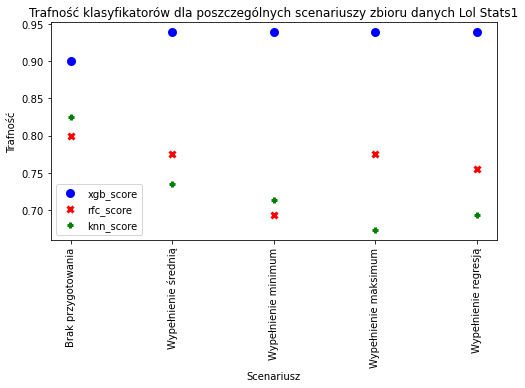
\includegraphics{Lol_Stats_1_Wypełnienie_brakujących}}
\centering
\caption{Trafność klasyfikatorów po wypełnieniu brakujących wartości dla zestawu danych Lol Stats 1}
\end{figure}

\begin{figure}[H]
\centerline{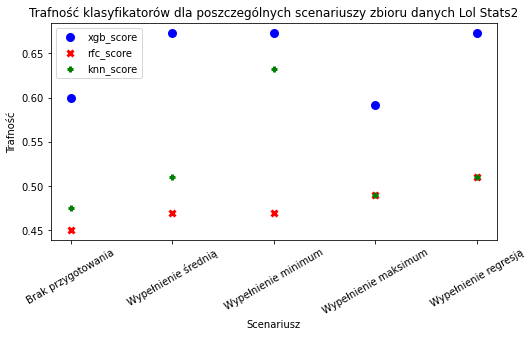
\includegraphics{Lol_Stats_2_Wypełnienie_brakujących}}
\centering
\caption{Trafność klasyfikatorów po wypełnieniu brakujących wartości dla zestawu danych Lol Stats 2}
\end{figure}

\begin{figure}[H]
\centerline{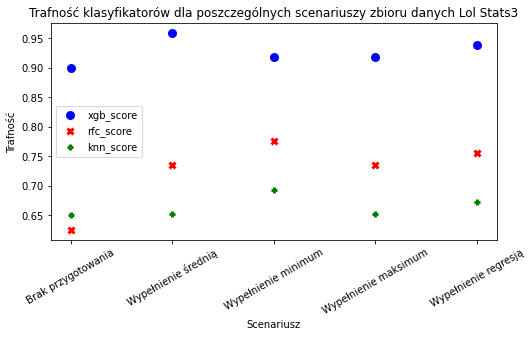
\includegraphics{Lol_Stats_3_Wypełnienie_brakujących}}
\centering
\caption{Trafność klasyfikatorów po wypełnieniu brakujących wartości dla zestawu danych Lol Stats 3}
\end{figure}


Dla klasyfikatora xgBoost wypełnienie jakąkolwiek wartością daje widoczną poprawę w trafności, 
jednak najlepsze wyniki uzyskujemy przy wartości średniej. Dla RandomForestClassifier uzyskujemy 
różne rezultaty w zależności od wygenerowanych dziur w zbiorze danych, w pierwszym przypadku jakiekolwiek 
wypełnianie pogarsza klasyfikację, w drugim regresja jest najlepszym sposobem, a w trzecim minimum. 
Dla algorytmu k-nearest neighbors w każdym z przypadków nie uzyskujemy poprawy albo wręcz pogarszamy wyniki przez 
wypełnienie brakujących wartości.

\subsection{Standaryzacja}

\begin{figure}[H]
\centerline{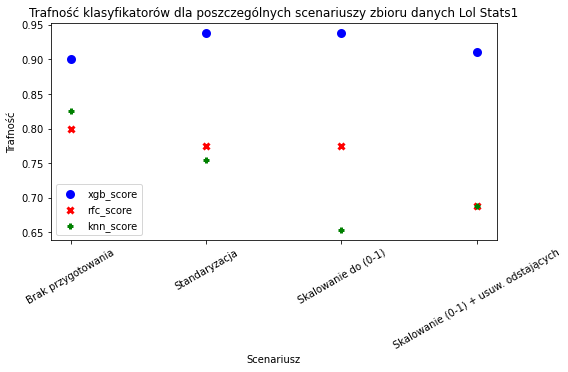
\includegraphics{Lol_Stats_1_Standaryzacja}}
\centering
\caption{Trafność klasyfikatorów po standaryzacji dla zestawu danych Lol Stats 1}
\end{figure}

\begin{figure}[H]
\centerline{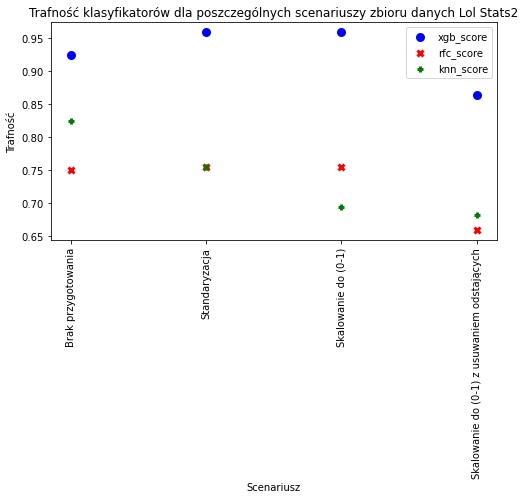
\includegraphics{Lol_Stats_2_Standaryzacja}}
\centering
\caption{Trafność klasyfikatorów po standaryzacji dla zestawu danych Lol Stats 2}
\end{figure}

\begin{figure}[H]
\centerline{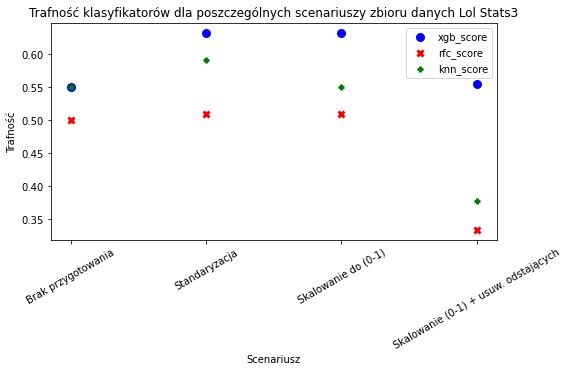
\includegraphics{Lol_Stats_3_Standaryzacja}}
\centering
\caption{Trafność klasyfikatorów po standaryzacji dla zestawu danych Lol Stats 3}
\end{figure}

Klasyfikator xgBoost osiąga niemalże perfekcję po 
standaryzacji lub standaryzacji ze skalowaniem do przedziału (0,1). 
Dla RandomForestClassifier jedynie w trzecim przypadku uzyskujemy poprawę przy 
standaryzacji oraz skalowaniu do przedziału (0,1) 
Dla algorytmu k-nearest neighbors podobnie jak dla RandomForestClassifier jedynie 
trzeci przypadek wykazuje poprawę trafności.
Należy zwrócić uwagę na fakt, że dla każdego z przypadków usunięcie wartości 
odstających znacznie pogarsza trafność klasyfikacji, 
nawet względem braku przygotowania danych

\subsection{Kodowanie}


\begin{figure}[H]
\centerline{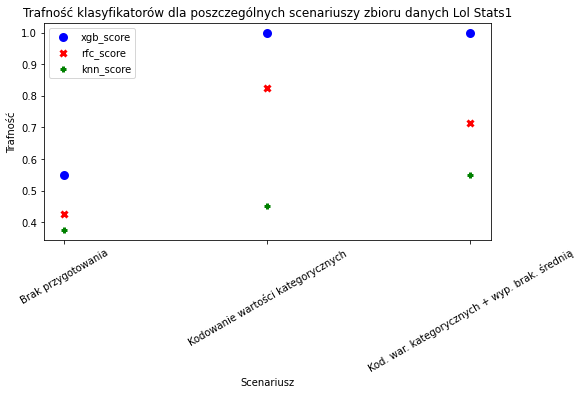
\includegraphics{Lol_Stats_1_Kodowanie}}
\centering
\caption{Trafność klasyfikatorów po kodowaniu dla zestawu danych Lol Stats 1}
\end{figure}

\begin{figure}[H]
\centerline{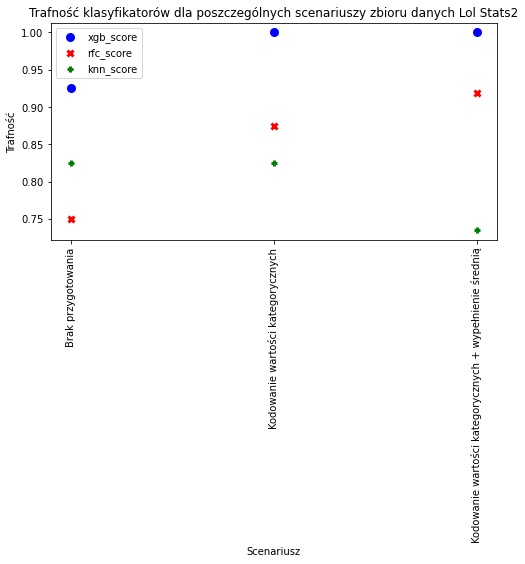
\includegraphics{Lol_Stats_2_Kodowanie}}
\centering
\caption{Trafność klasyfikatorów po kodowaniu dla zestawu danych Lol Stats 2}
\end{figure}

\begin{figure}[H]
\centerline{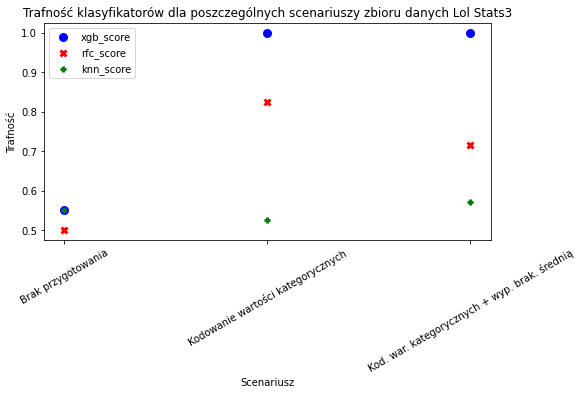
\includegraphics{Lol_Stats_3_Kodowanie}}
\centering
\caption{Trafność klasyfikatorów po kodowaniu dla zestawu danych Lol Stats 3}
\end{figure}

XgBoost po kodowaniu wartości kategorycznych osiąga perfekcję i utrzymuje się na tym poziomie, 
RandomForestClassifier dla samego kodowania wykazuje poprawę we wszystkich przypadkach, 
natomiast dla pierwszego przypadku wypełnienie brakujacych wartości średnią powoduje 
pogorszenie wyników względem samego kodowania. Dla algorytmu k-nearest neighbors poprawa uzyskana 
dzięki kodowaniu jest nieznaczna, jednak bardzo często w połączeniu z wypełenieniem wartości brakujących 
średnią uzyskujemy wynik gorszy od braku przygotowania.

\subsection{Indywidualne podejście}

\begin{figure}[H]
\centerline{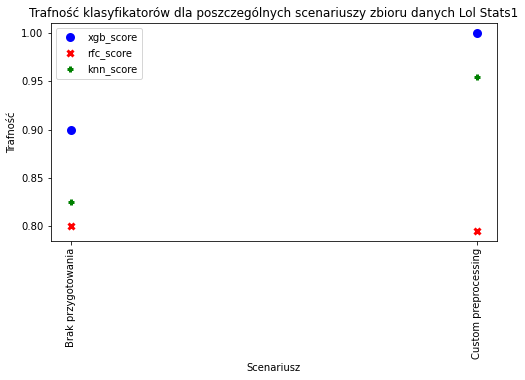
\includegraphics{Lol_Stats_1_Custom}}
\centering
\caption{Trafność klasyfikatorów po indywidualnym podejśćiu dla zestawu danych Lol Stats 1}
\end{figure}

\begin{figure}[H]
\centerline{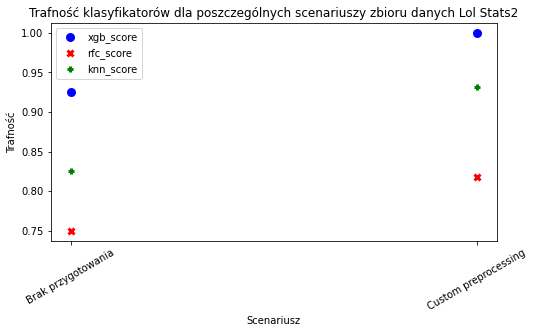
\includegraphics{Lol_Stats_2_Custom}}
\centering
\caption{Trafność klasyfikatorów po indywidualnym podejśćiu dla zestawu danych Lol Stats 2}
\end{figure}

\begin{figure}[H]
\centerline{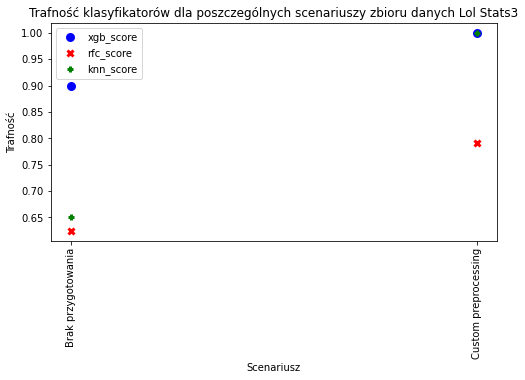
\includegraphics{Lol_Stats_3_Custom}}
\centering
\caption{Trafność klasyfikatorów po indywidualnym podejśćiu dla zestawu danych Lol Stats 3}
\end{figure}



\section{Australian Rain Forecast}


\subsection{Wypełnienie brakujących wartości}
\begin{figure}[H]
\centerline{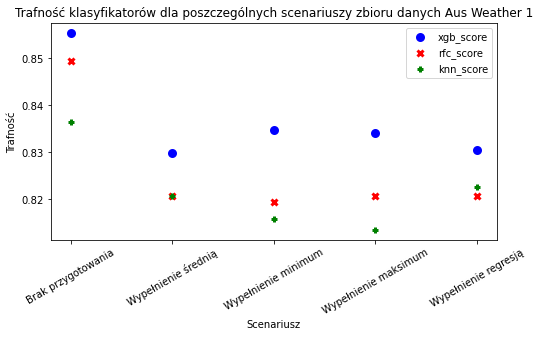
\includegraphics{Aus_Weather_1_Wypełnienie_brakujących}}
\centering
\caption{Trafność klasyfikatorów po przygotowaniu danych 
według danego scenariusza}
\end{figure}

\begin{figure}[H]
\centerline{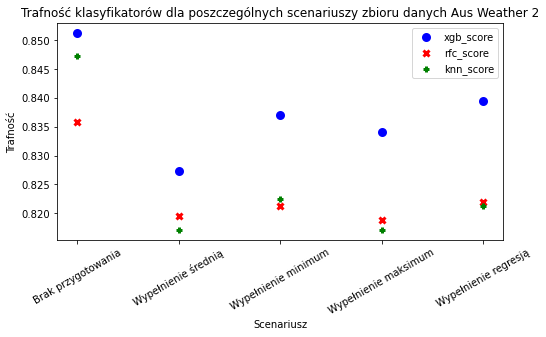
\includegraphics{Aus_Weather_2_Wypełnienie_brakujących}}
\centering
\caption{Trafność klasyfikatorów po przygotowaniu danych 
według danego scenariusza}
\end{figure}

\begin{figure}[H]
\centerline{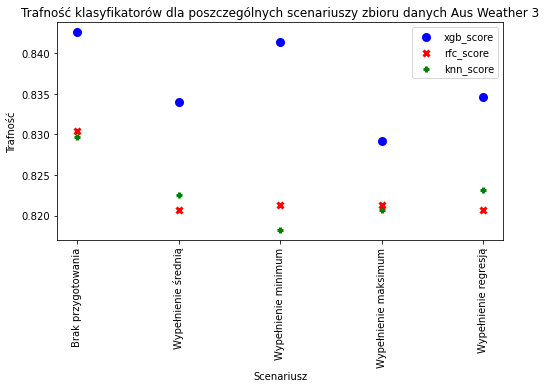
\includegraphics{Aus_Weather_3_Wypełnienie_brakujących}}
\centering
\caption{Trafność klasyfikatorów po przygotowaniu danych 
według danego scenariusza}
\end{figure}

\subsection{Standaryzacja}

\begin{figure}[H]
\centerline{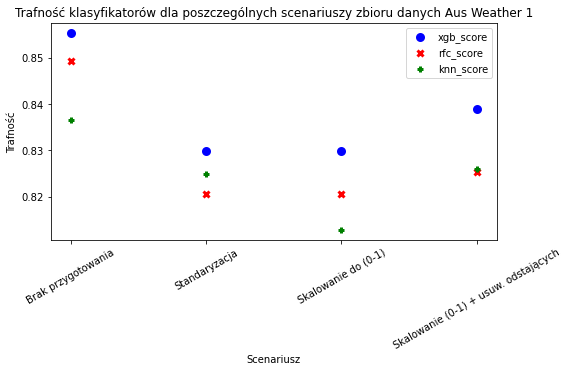
\includegraphics{Aus_Weather_1_Standaryzacja}}
\centering
\caption{Trafność klasyfikatorów po przygotowaniu danych 
według danego scenariusza}
\end{figure}

\begin{figure}[H]
\centerline{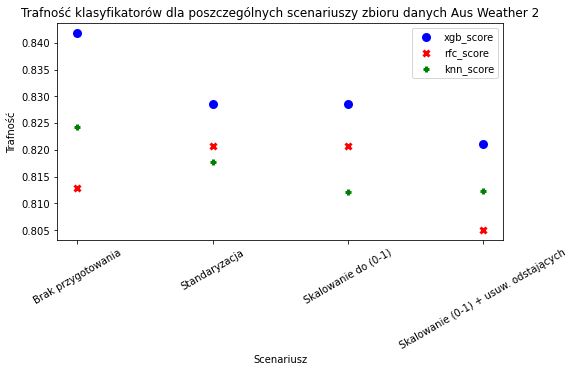
\includegraphics{Aus_Weather_2_Standaryzacja}}
\centering
\caption{Trafność klasyfikatorów po przygotowaniu danych 
według danego scenariusza}
\end{figure}

\begin{figure}[H]
\centerline{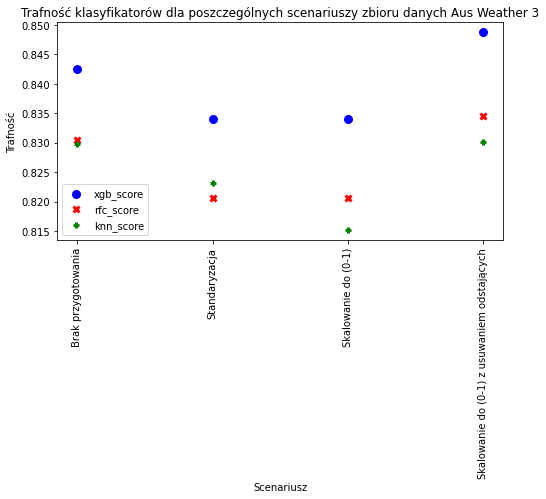
\includegraphics{Aus_Weather_3_Standaryzacja}}
\centering
\caption{Trafność klasyfikatorów po przygotowaniu danych 
według danego scenariusza}
\end{figure}

\subsection{Kodowanie}


\begin{figure}[H]
\centerline{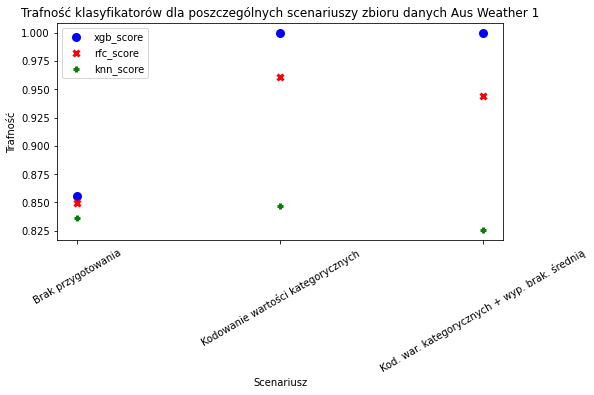
\includegraphics{Aus_Weather_1_Kodowanie}}
\centering
\caption{Trafność klasyfikatorów po przygotowaniu danych 
według danego scenariusza}
\end{figure}

\begin{figure}[H]
\centerline{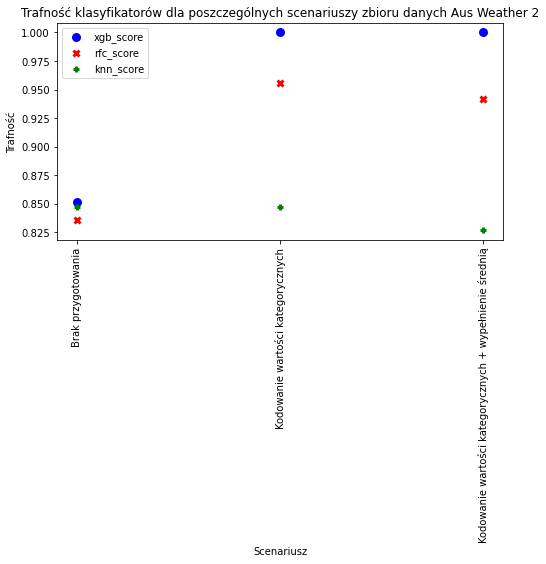
\includegraphics{Aus_Weather_2_Kodowanie}}
\centering
\caption{Trafność klasyfikatorów po przygotowaniu danych 
według danego scenariusza}
\end{figure}

\begin{figure}[H]
\centerline{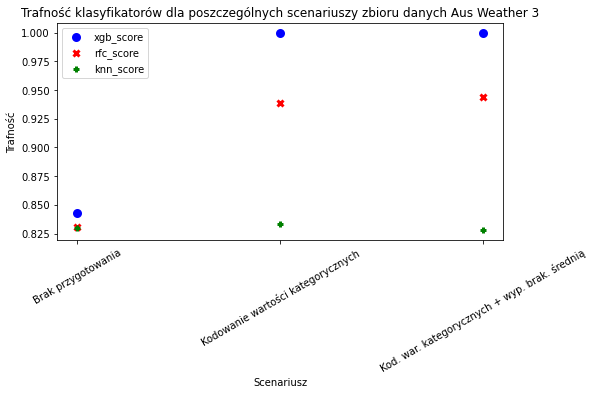
\includegraphics{Aus_Weather_3_Kodowanie}}
\centering
\caption{Trafność klasyfikatorów po przygotowaniu danych 
według danego scenariusza}
\end{figure}

\subsection{Indywidualne podejście}

\begin{figure}[H]
\centerline{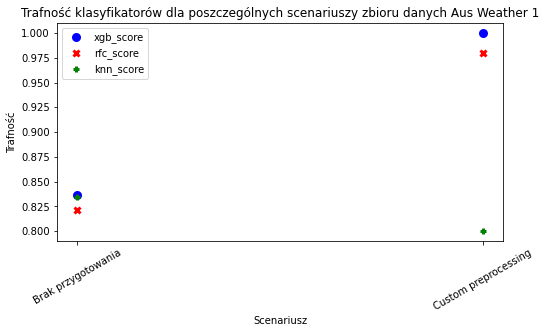
\includegraphics{Aus_Weather_1_Custom}}
\centering
\caption{Trafność klasyfikatorów po przygotowaniu danych 
według danego scenariusza}
\end{figure}

\begin{figure}[H]
\centerline{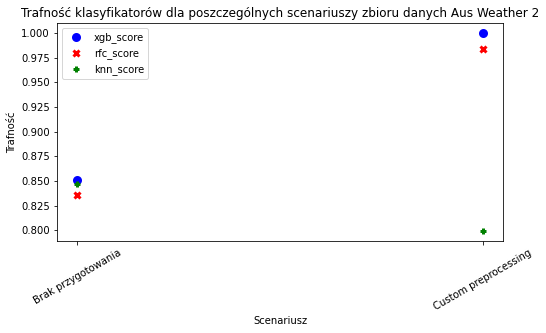
\includegraphics{Aus_Weather_2_Custom}}
\centering
\caption{Trafność klasyfikatorów po przygotowaniu danych 
według danego scenariusza}
\end{figure}

\begin{figure}[H]
\centerline{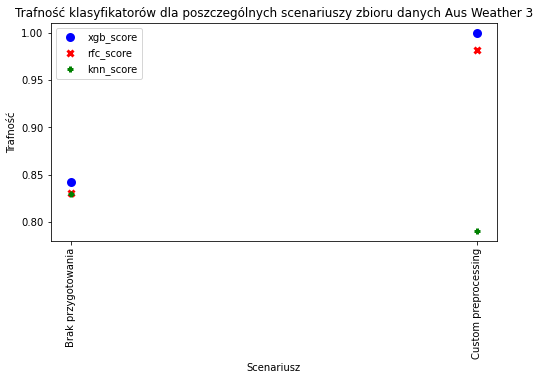
\includegraphics{Aus_Weather_3_Custom}}
\centering
\caption{Trafność klasyfikatorów po przygotowaniu danych 
według danego scenariusza}
\end{figure}


\section{Titanic Survival}


\subsection{Wypełnienie brakujących wartości}
\begin{figure}[H]
\centerline{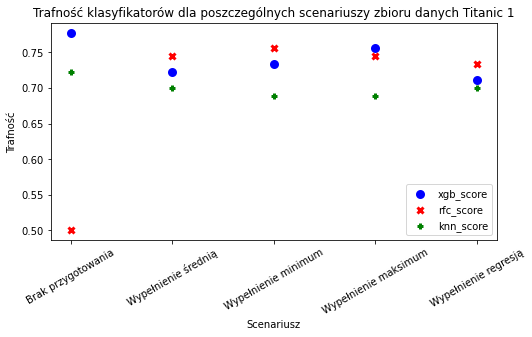
\includegraphics{Titanic_1_Wypełnienie_brakujących}}
\centering
\caption{Trafność klasyfikatorów po przygotowaniu danych 
według danego scenariusza}
\end{figure}

\begin{figure}[H]
\centerline{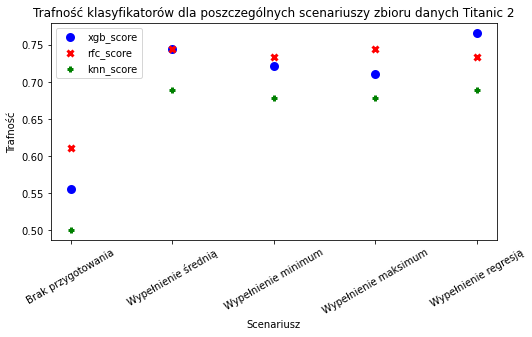
\includegraphics{Titanic_2_Wypełnienie_brakujących}}
\centering
\caption{Trafność klasyfikatorów po przygotowaniu danych 
według danego scenariusza}
\end{figure}

\begin{figure}[H]
\centerline{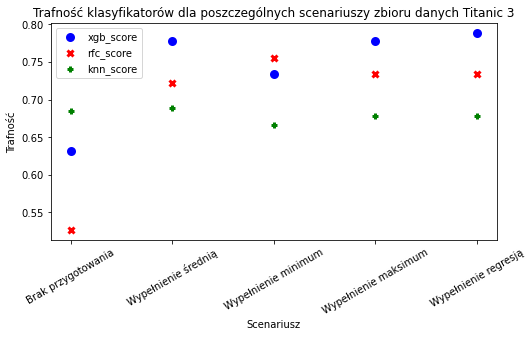
\includegraphics{Titanic_3_Wypełnienie_brakujących}}
\centering
\caption{Trafność klasyfikatorów po przygotowaniu danych 
według danego scenariusza}
\end{figure}

\subsection{Standaryzacja}

\begin{figure}[H]
\centerline{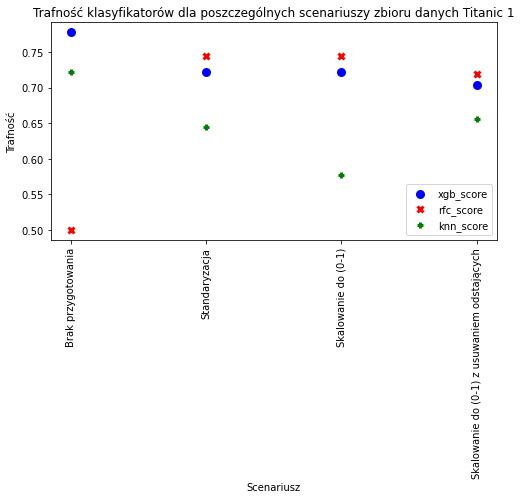
\includegraphics{Titanic_1_Standaryzacja}}
\centering
\caption{Trafność klasyfikatorów po przygotowaniu danych 
według danego scenariusza}
\end{figure}

\begin{figure}[H]
\centerline{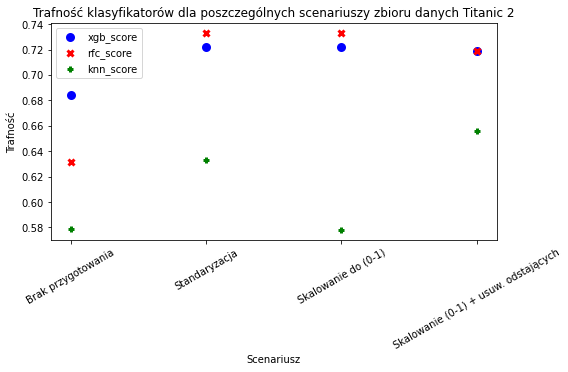
\includegraphics{Titanic_2_Standaryzacja}}
\centering
\caption{Trafność klasyfikatorów po przygotowaniu danych 
według danego scenariusza}
\end{figure}

\begin{figure}[H]
\centerline{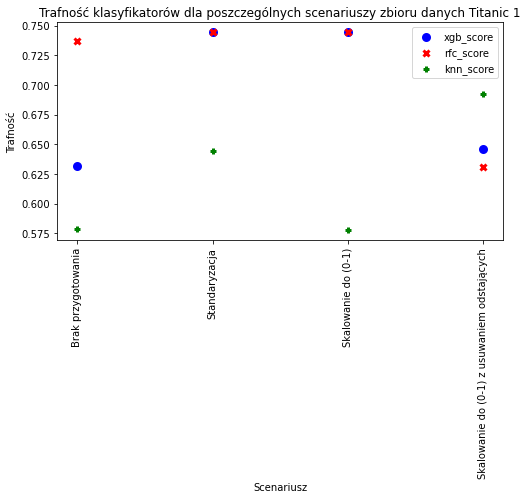
\includegraphics{Titanic_3_Standaryzacja}}
\centering
\caption{Trafność klasyfikatorów po przygotowaniu danych 
według danego scenariusza}
\end{figure}

\subsection{Kodowanie}


\begin{figure}[H]
\centerline{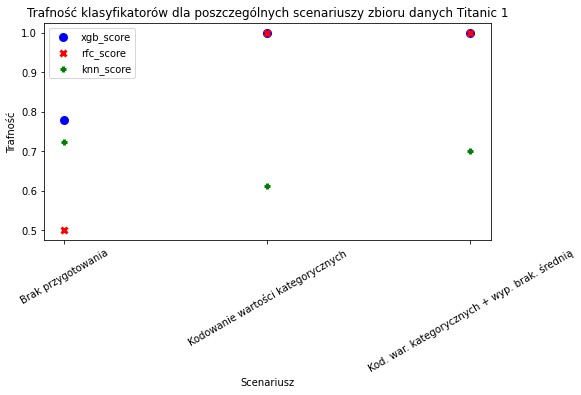
\includegraphics{Titanic_1_Kodowanie}}
\centering
\caption{Trafność klasyfikatorów po przygotowaniu danych 
według danego scenariusza}
\end{figure}

\begin{figure}[H]
\centerline{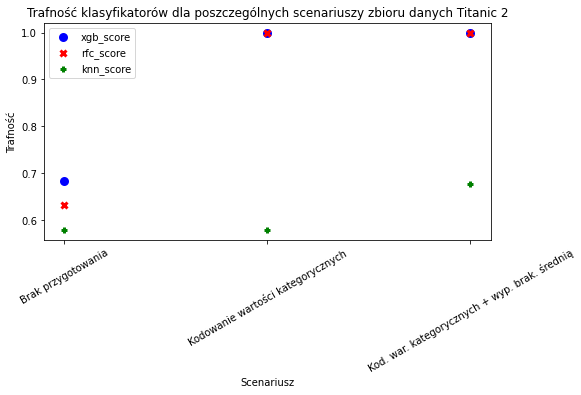
\includegraphics{Titanic_2_Kodowanie}}
\centering
\caption{Trafność klasyfikatorów po przygotowaniu danych 
według danego scenariusza}
\end{figure}

\begin{figure}[H]
\centerline{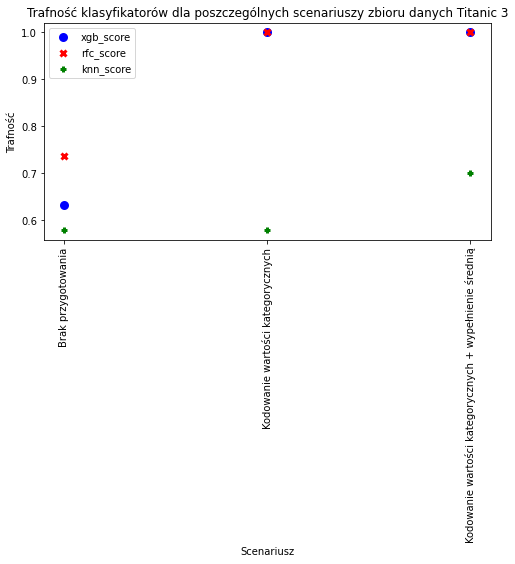
\includegraphics{Titanic_3_Kodowanie}}
\centering
\caption{Trafność klasyfikatorów po przygotowaniu danych 
według danego scenariusza}
\end{figure}

\subsection{Indywidualne podejście}

\begin{figure}[H]
\centerline{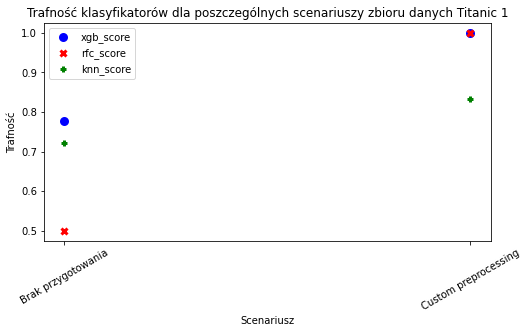
\includegraphics{Titanic_1_Custom}}
\centering
\caption{Trafność klasyfikatorów po przygotowaniu danych 
według danego scenariusza}
\end{figure}

\begin{figure}[H]
\centerline{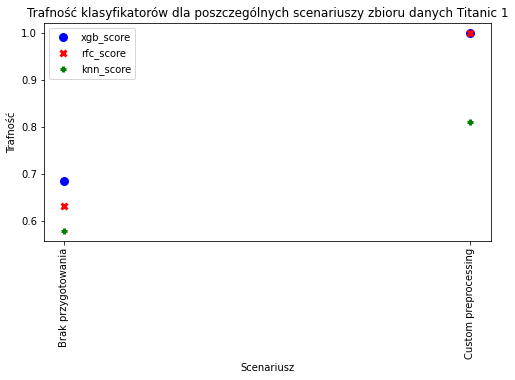
\includegraphics{Titanic_2_Custom}}
\centering
\caption{Trafność klasyfikatorów po przygotowaniu danych 
według danego scenariusza}
\end{figure}

\begin{figure}[H]
\centerline{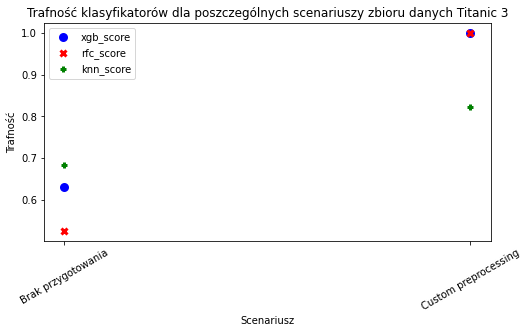
\includegraphics{Titanic_3_Custom}}
\centering
\caption{Trafność klasyfikatorów po przygotowaniu danych 
według danego scenariusza}
\end{figure}


\section{Średnie wyniki}


\chapter{Podsumowanie}
Z przeprowadzonych eksperymentów wynika, 
że odpowiednie przygotowanie danych zwiększa trafność 
klasyfikatorów. Należy jednak zwrócić uwagę, że nie wszystkie 
scenariusze skutkowały jednoznaczną poprawą rezultatów. 
Na szczególne wyróżenienie zasługuje kodowanie wartości 
kategorycznych na liczbowe, gdyż w każdym przypadku zastosowanie 
tej metody znacznie zwiększyło trafność klasyfikacji

\begin{thebibliography}{9}
    \bibitem{data_analysis}
    \href{https://www.intel.pl/content/www/pl/pl/analytics/resources/what-is-data-analytics.html}{Definicja zaproponowana przez firmę Intel}
    \bibitem{titanic_dataset}
    \href{https://www.kaggle.com/competitions/titanic/data?select=train.csv}{Zbiór danych Titanic dostępny do pobrania ze strony kaggle.com}
    \bibitem{lol_stats_dataset}
    \href{https://www.kaggle.com/datasets/vivovinco/league-of-legends-stats-s13}{Zbiór danych Lol Stats dostępny do pobrania ze strony kaggle.com}
    \bibitem{australian_rain_dataset}
    \href{https://www.kaggle.com/datasets/jsphyg/weather-dataset-rattle-package}{Zbiór danych Australian Rain dostępny do pobrania ze strony kaggle.com}
    
    \bibitem{lamport94}
    Leslie Lamport (1994) \emph{\LaTeX: a document preparation system}, Addison
    Wesley, Massachusetts, 2nd ed.
    \end{thebibliography}


\end{document}